\label{sec:result_analysis}

We evaluated the proposed resolution strategy on seven distinct workpieces: a stair step of a spiral staircase, a stair step of a simple staircase, a music speaker, a dashboard, a coffee table, a door, and a door with a porthole (see Table~\ref{tab:visual_results}).

The work center considered was equipped with 24 square fixtures with dimensions \(145 \times 145\)~mm and 12 rectangular fixtures with dimensions \(180 \times 65\)~mm. The minimum and maximum numbers of fixtures were set to \(\nmin = 3\) and \(\nmax = 6\), respectively, for all workpieces except the coffee table and the two door workpieces, which, due to their larger dimensions, required \(\nmin = 6\) and \(\nmax = 10\), and \(\nmin = 10\) and \(\nmax = 20\), respectively.

Both the CP and MIP models were implemented in \textit{MiniZinc} version~2.9.5~\cite{nethercote2007MiniZinc}. The CP model was solved using the CP solvers Gecode~\cite{schulte2006gecode}, Chuffed~\cite{chuffed}, and OR-Tools~\cite{ortools}, whereas the MIP model was solved using the commercial solver Gurobi~\cite{gurobi}.

We also considered \(\lns\), a variant of Gecode implementing Large Neighborhood Search (LNS)~\cite{pisinger2018large}, to solve the CP model, configuring it to explore the search space by randomly fixing 80\% of the decision variables corresponding to the \(x\)- and \(y\)-coordinates, adopting a constant restart strategy triggered every 1000 explored nodes.

All solvers were executed in single-threaded mode to ensure a fair comparison. The experiments were performed on a 64-bit Windows machine equipped with an Intel Core i5 processor and 16~GB of RAM.

\begin{table}[!b]
	\centering
	\footnotesize
	\caption{Objective values for $\fdist$ and $\finer$, and solve time $t_{solve}$ in seconds to reach the best $\fdist$ solution. Timeout (300~s) is indicated by ``--''. Solutions where the solver reached optimality are marked with $^*$. For each workpiece, the maximum values of $\fdist$ and $\finer$ are highlighted in bold, including ties.}
	\label{tab:objective_runtime}
	\setlength{\tabcolsep}{2pt}
	\begin{tabular}{llccccc}
		\toprule
		Workpiece & Metric & Gecode & \lns & Chuffed & OR-Tools & Gurobi \\
		\midrule
		
		\multirow{3}{*}{\makecell{Stair step\\spiral staircase}} & $\fdist$ & $45655{}^*$ & $45655$ & $45655{}^*$ & $45655{}^*$ & $\mathbf{45662.155{}^*}$ \\
		& $\finer$ & \cellcolor{gray!15}$2.13968\times 10^{9}$ & \cellcolor{gray!15}$2.13968\times 10^{9}$ & \cellcolor{gray!15}$2.13960\times 10^{9}$ & \cellcolor{gray!15}$2.13968\times 10^{9}$ & \cellcolor{gray!15}$\mathbf{2.17089\times 10^{9}}$ \\
		& $t_{solve}$ & 0.559 & -- & 0.326 & 0.120 & 2.930 \\
		\midrule
		
		\multirow{3}{*}{\makecell{Stair step\\simple staircase}} & $\fdist$ & $72823$ & $72823$ & $72823{}^*$ & $72721$ & $\mathbf{72826.000{}^*}$ \\
		& $\finer$ & \cellcolor{gray!15}$6.76573\times 10^{9}$ & \cellcolor{gray!15}$6.76573\times 10^{9}$ & \cellcolor{gray!15}$6.76530\times 10^{9}$ & \cellcolor{gray!15}$6.48172\times 10^{9}$ & \cellcolor{gray!15}$\mathbf{6.76638\times 10^{9}}$ \\
		& $t_{solve}$ & -- & -- & 3.386 & -- & 0.220 \\
		\midrule
		
		\multirow{3}{*}{\makecell{Dashboard}} & $\fdist$ & $\mathbf{55582{}^*}$ & $\mathbf{55582}$ & $\mathbf{55582{}^*}$ & $\mathbf{55582{}^*}$ & $\mathbf{55582.000{}^*}$ \\
		& $\finer$ & \cellcolor{gray!15}$\mathbf{7.10094\times 10^{9}}$ & \cellcolor{gray!15}$\mathbf{7.10094\times 10^{9}}$ & \cellcolor{gray!15}$7.08735\times 10^{9}$ & \cellcolor{gray!15}$7.08735\times 10^{9}$ & \cellcolor{gray!15}$7.08735\times 10^{9}$ \\
		& $t_{solve}$ & 0.044 & -- & 0.057 & 0.102 & 0.157 \\
		\midrule
		
		\multirow{3}{*}{\makecell{Speaker}} & $\fdist$ & $\mathbf{49548{}^*}$ & $\mathbf{49548}$ & $\mathbf{49548{}^*}$ & $\mathbf{49548{}^*}$ & $\mathbf{49548.000{}^*}$ \\
		& $\finer$ & \cellcolor{gray!15}$\mathbf{2.93433\times 10^{9}}$ & \cellcolor{gray!15}$\mathbf{2.93433\times 10^{9}}$ & \cellcolor{gray!15}$\mathbf{2.93433\times 10^{9}}$ & \cellcolor{gray!15}$\mathbf{2.93433\times 10^{9}}$ & \cellcolor{gray!15}$\mathbf{2.93433\times 10^{9}}$ \\
		& $t_{solve}$ & 165.018 & -- & 0.106 & 0.120 & 0.126 \\
		\midrule
		
		\multirow{3}{*}{\makecell{Coffee table}} & $\fdist$ & $137262$ & $185351$ & $192711$ & $122920$ & $\mathbf{201686.505}$ \\
		& $\finer$ & \cellcolor{gray!15}$2.20750\times 10^{10}$ & \cellcolor{gray!15}$2.19967\times 10^{10}$ & \cellcolor{gray!15}$\mathbf{2.21449\times 10^{10}}$ & \cellcolor{gray!15}$9.10490\times 10^{9}$ & \cellcolor{gray!15}$2.19472\times 10^{10}$ \\
		& $t_{solve}$ & -- & -- & -- & -- & -- \\
		\midrule
		
		\multirow{3}{*}{\makecell{Door}} & $\fdist$ & $261757$ & $\mathbf{521632}$ & -- & -- & $355744.000$ \\
		& $\finer$ & \cellcolor{gray!15}$1.08442\times 10^{11}$ & \cellcolor{gray!15}$\mathbf{1.52925\times 10^{11}}$ & \cellcolor{gray!15}-- & \cellcolor{gray!15}-- & \cellcolor{gray!15}$1.17690\times 10^{11}$ \\
		& $t_{solve}$ & -- & -- & -- & -- & -- \\
		\midrule
		
		\multirow{3}{*}{\makecell{Door\\with porthole}} & $\fdist$ & $261759$ & $\mathbf{393343}$ & -- & -- & $298186.000$ \\
		& $\finer$ & \cellcolor{gray!15}$1.08422\times 10^{11}$ & \cellcolor{gray!15}$\mathbf{1.52861\times 10^{11}}$ & \cellcolor{gray!15}-- & \cellcolor{gray!15}-- & \cellcolor{gray!15}$1.39714\times 10^{11}$ \\
		& $t_{solve}$ & -- & -- & -- & -- & -- \\
		
		\bottomrule
	\end{tabular}
\end{table}


%\begin{table}[t]
%	\centering
%	\footnotesize
%	\caption{Objective values for $\fdist$ and $\finer$. Solutions where the solver reached optimality (runtime $< 300$ s) are marked with $^*$. For each workpiece, the maximum values of $\fdist$ and $\finer$ are highlighted in bold, including ties. Note that solutions equivalent in terms of $\fdist$ may differ in $\finer$, hence different entries may be highlighted.}
%	\label{tab:objective}
%	\setlength{\tabcolsep}{2pt}
%	\begin{tabular}{llccccc}
%		\toprule
%		Workpiece & Obj. & Gecode & \lns & Chuffed & OR-Tools & Gurobi \\
%		\midrule
%		
%		\multirow{2}{*}{\makecell{Stair step\\spiral staircase}} & $\fdist$ & 45655$^*$ & 45655 & 45655$^*$ & 45655$^*$ & \textbf{45662.155}$^*$ \\
%		& $\finer$ & \cellcolor{gray!15}$2.13968\times 10^{9}$ & \cellcolor{gray!15}$2.13968\times 10^{9}$ & \cellcolor{gray!15}$2.13960\times 10^{9}$ & \cellcolor{gray!15}$2.13968\times 10^{9}$ & \cellcolor{gray!15}$\mathbf{2.17089\times 10^{9}}$ \\
%		\midrule
%		
%		\multirow{2}{*}{\makecell{Stair step\\simple staircase}} & $\fdist$ & 72823 & 72823 & 72823$^*$ & 72721 & \textbf{72826}$^*$ \\
%		& $\finer$ & \cellcolor{gray!15}$6.76573\times 10^{9}$ & \cellcolor{gray!15}$6.76573\times 10^{9}$ & \cellcolor{gray!15}$6.76530\times 10^{9}$ & \cellcolor{gray!15}$6.48172\times 10^{9}$ & \cellcolor{gray!15}$\mathbf{6.76638\times 10^{9}}$ \\
%		\midrule
%		
%		\multirow{2}{*}{\makecell{Dashboard}} & $\fdist$ & \textbf{55582}$^*$ & \textbf{55582} & \textbf{55582}$^*$ & \textbf{55582}$^*$ & \textbf{55582}$^*$ \\
%		& $\finer$ & \cellcolor{gray!15}$\mathbf{7.10094\times 10^{9}}$ & \cellcolor{gray!15}$\mathbf{7.10094\times 10^{9}}$ & \cellcolor{gray!15}$7.08735\times 10^{9}$ & \cellcolor{gray!15}$7.08735\times 10^{9}$ & \cellcolor{gray!15}$7.08735\times 10^{9}$ \\
%		\midrule
%		
%		\multirow{2}{*}{\makecell{Speaker}} & $\fdist$ & \textbf{49548}$^*$ & \textbf{49548} & \textbf{49548}$^*$ & \textbf{49548}$^*$ & \textbf{49548}$^*$\\
%		& $\finer$ & \cellcolor{gray!15}$\mathbf{2.93433\times 10^{9}}$ & \cellcolor{gray!15}$\mathbf{2.93433\times 10^{9}}$ & \cellcolor{gray!15}$\mathbf{2.93433\times 10^{9}}$ & \cellcolor{gray!15}$\mathbf{2.93433\times 10^{9}}$ & \cellcolor{gray!15}$\mathbf{2.93433\times 10^{9}}$ \\
%		\midrule
%		
%		\multirow{2}{*}{\makecell{Coffee table}} & $\fdist$ & 137262 & 185351 & 192711 & 122920 & \textbf{201686.505} \\
%		& $\finer$ & \cellcolor{gray!15}$2.20750\times 10^{10}$ & \cellcolor{gray!15}$2.19967\times 10^{10}$ & \cellcolor{gray!15}$\mathbf{2.21449\times 10^{10}}$ & \cellcolor{gray!15}$9.10490\times 10^{9}$ & \cellcolor{gray!15}$2.19472\times 10^{10}$ \\
%		\midrule
%		
%		\multirow{2}{*}{\makecell{Door}} & $\fdist$ & 261757 & \textbf{521632} & -- & -- & 355744 \\
%		& $\finer$ & \cellcolor{gray!15}$1.08442\times 10^{11}$ & \cellcolor{gray!15}$\mathbf{1.52925\times 10^{11}}$ & \cellcolor{gray!15}-- & \cellcolor{gray!15}-- & \cellcolor{gray!15}$1.17690\times 10^{11}$ \\
%		\midrule
%		
%		\multirow{2}{*}{\makecell{Door\\with porthole}} & $\fdist$ & 261759 & \textbf{393343} & -- & -- & 298186 \\
%		& $\finer$ & \cellcolor{gray!15}$1.08422\times 10^{11}$ & \cellcolor{gray!15}$\mathbf{1.52861\times 10^{11}}$ & \cellcolor{gray!15}-- & \cellcolor{gray!15}-- & \cellcolor{gray!15}$1.39714\times 10^{11}$ \\
%		
%		\bottomrule
%	\end{tabular}
%\end{table}

%\begin{table}[t]
%	\centering
%	\footnotesize
%	\caption{Solve time in seconds to reach the best $\fdist$ solution. Timeout (300~s) is indicated by ``--''.}
%	\label{tab:runtime}
%	%\rowcolors{2}{gray!15}{white}
%	\begin{tabular}{cccccc}
	%		\toprule
	%		Workpiece & Gecode & \lns & Chuffed & OR-Tools & Gurobi \\
	%		\midrule
	%		
	%		\makecell{Stair step\\spiral staircase} & 0.559 & -- & 0.326 & 0.120 & 2.930 \\
	%		\midrule
	%		
	%		\makecell{Stair step\\simple staircase} & -- & -- & 3.386 & -- & 0.220 \\
	%		\midrule
	%		
	%		\makecell{Dashboard} & 0.044 & -- & 0.057 & 0.102 & 0.157 \\
	%		\midrule
	%		
	%		\makecell{Speaker} & 165.018 & -- & 0.106 & 0.120 & 0.126 \\
	%		\midrule
	%		
	%		\makecell{Coffee table} & -- & -- & -- & -- & -- \\
	%		\midrule
	%		
	%		\makecell{Door} & -- & -- & -- & -- & -- \\
	%		\midrule
	%		
	%		\makecell{Door\\with porthole} & -- & -- & -- & -- & -- \\
	%		
	%		\bottomrule
	%	\end{tabular}
%\end{table}

Table~\ref{tab:objective_runtime} reports the values obtained for the objective function $\fdist$ for the different workpieces, together with the corresponding \emph{a posteriori} values of $\finer$, and the solve time $t_{solve}$ required to reach the optimal solution. 

Identical values of $\fdist$ do not necessarily correspond to identical values of $\finer$, as observed for the Dashboard workpiece. This is because the moments of inertia are highly sensitive to little displacement; therefore, if the solutions obtained by the solvers do not result in identical fixture placements, the value of $\finer$ may differ. 

Among the CP solvers, Gecode delivers the best overall performance, finding feasible solutions for all the considered workpieces, whereas Chuffed and OR-Tools fail to find feasible solutions for the two door workpieces.

$\lns$ achieves the best results for the two door workpieces, producing layouts that outperform those obtained by Gurobi with the MIP model. For the remaining workpieces, however, Gurobi finds solutions that are either superior or equivalent to those obtained by the CP solvers with respect to $\fdist$. This can be partly attributed to the use of continuous decision variables in the MIP model, which enlarges the feasible region and may therefore yield higher-quality solutions.

If we consider the information of the solve time presented in Table~\ref{tab:objective_runtime}, among the CP solvers, with an imposed time limit of 300~s, Chuffed is the most robust, finding the optimal solution in four of the seven instances, and it is the only CP solver able to prove optimality for the stiar step of the simple staircase. Gecode exhibits the greatest variability in performance, ranging from competitive runtimes on the easier instances to requiring 165.018~s for the speaker workpiece, while Chuffed and OR-Tools solve the same instance in only 0.106~s and 0.120~s, respectively.

Being a local-search-based approach, $\lns$ cannot prove optimality. Nevertheless, it reaches the same optimal value of $\fdist$ as the other CP solvers for the simpler workpieces and achieves the best value of $\finer$ in four out of the seven considered workpieces, demonstrating the effectiveness of a local search strategy.

The Q-learning-based algorithm was implemented in Python~3.11.9 using the Gymnasium library version~1.3.0. The agent was trained on all the considered workpieces for 200 episodes, each consisting of 20 steps, using the following hyperparameters: learning rate $\alpha = 0.1$, discount factor $\gamma = 0.99$, initial exploration rate $\epsilon = 1.0$, and exploration decay factor $\rho = 0.995$.

Table~\ref{tab:comparison} reports the results obtained for the different workpieces, comparing the corresponding values of the moment of inertia with those achieved by the best CP solver and the MIP model.

Overall, the Q-learning-based algorithm does not outperform either the CP or the MIP model. On average, the values of $\finer$ obtained by RL are 13\% lower than those achieved by CP and 8\% lower than those obtained with MIP. The only exception is the door with a porthole workpiece, for which Q-learning outperforms the solution returned by Gurobi for the MIP model.


\begin{table}[t]
	\centering
	\footnotesize
	\caption{Objective values $\finer$ comparison: CP solvers (best among Gecode, LNS, Chuffed, OR-Tools), MIP solver (Gurobi), and RL approach. For each workpiece, the maximum value is highlighted in bold.}
	\label{tab:comparison}
	\setlength{\tabcolsep}{5pt}
	\begin{tabular}{cccc}
		\toprule
		Workpiece & CP model & MIP model & Q-learning \\
		\midrule
		
		\makecell{Stair step\\spiral staircase} & $2.13968\times 10^{9}$ & $\mathbf{2.17089\times 10^{9}}$ & $1.93822\times 10^{9}$ \\
		\midrule
		
		\makecell{Stair step\\simple staircase} & $6.76573\times 10^{9}$ & $\mathbf{6.76638\times 10^{9}}$ & $5.65433\times 10^{9}$ \\
		\midrule
		
		\makecell{Dashboard} & $\mathbf{7.10094\times 10^{9}}$ & $7.08735\times 10^{9}$ & $6.65446\times 10^{9}$ \\
		\midrule
		
		\makecell{Speaker} & $\mathbf{2.93433\times 10^{9}}$ & $\mathbf{2.93433\times 10^{9}}$ & $2.81248\times 10^{9}$ \\
		\midrule
		
		\makecell{Coffee table} & $\mathbf{2.29750\times 10^{10}}$ & $2.19472\times 10^{10}$ & $1.56444\times 10^{10}$ \\
		\midrule
		
		\makecell{Door} & $\mathbf{1.52925\times 10^{11}}$ & $1.17690\times 10^{11}$ & $1.14387\times 10^{11}$ \\
		\midrule
		
		\makecell{Door\\with porthole} & $\mathbf{1.52861\times 10^{11}}$ & $1.39714\times 10^{11}$ & $1.45467\times 10^{11}$ \\
		
		\bottomrule
	\end{tabular}
\end{table}


\begin{figure}[t]
	\centering
	\begin{subfigure}[b]{\textwidth}
		\centering
		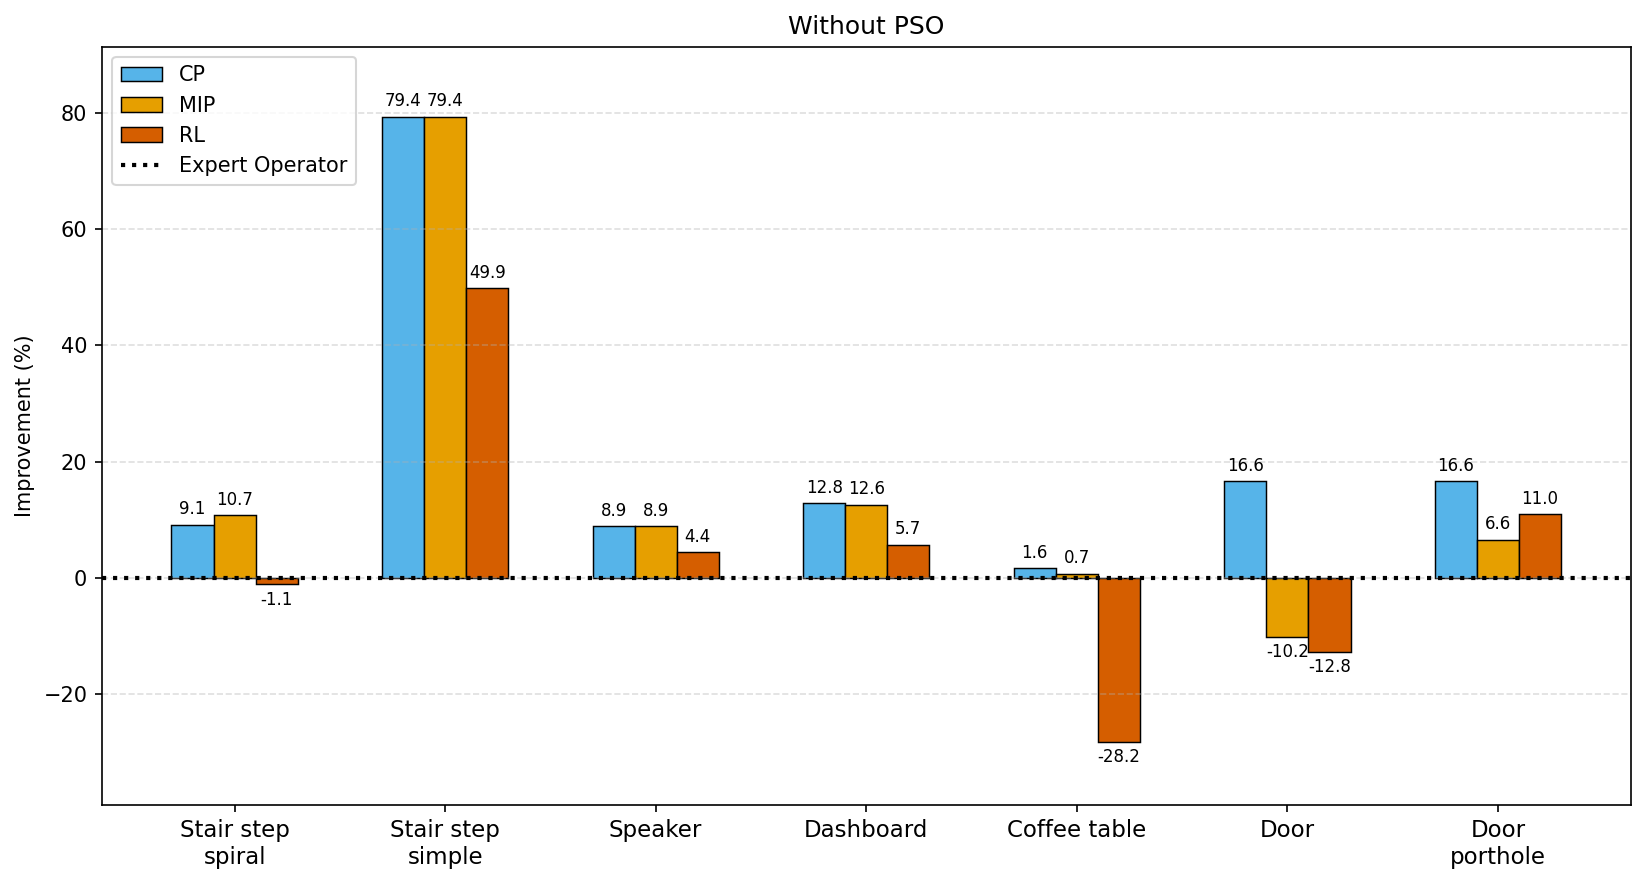
\includegraphics[width=0.7\textwidth]{img/comparison_plot_1.png}
		\caption{Percentage improvement over expert operator}
		\label{fig:comparison_plot1}
	\end{subfigure}
	%\hspace{1.5cm}
	\begin{subfigure}[b]{\textwidth}
		\centering
		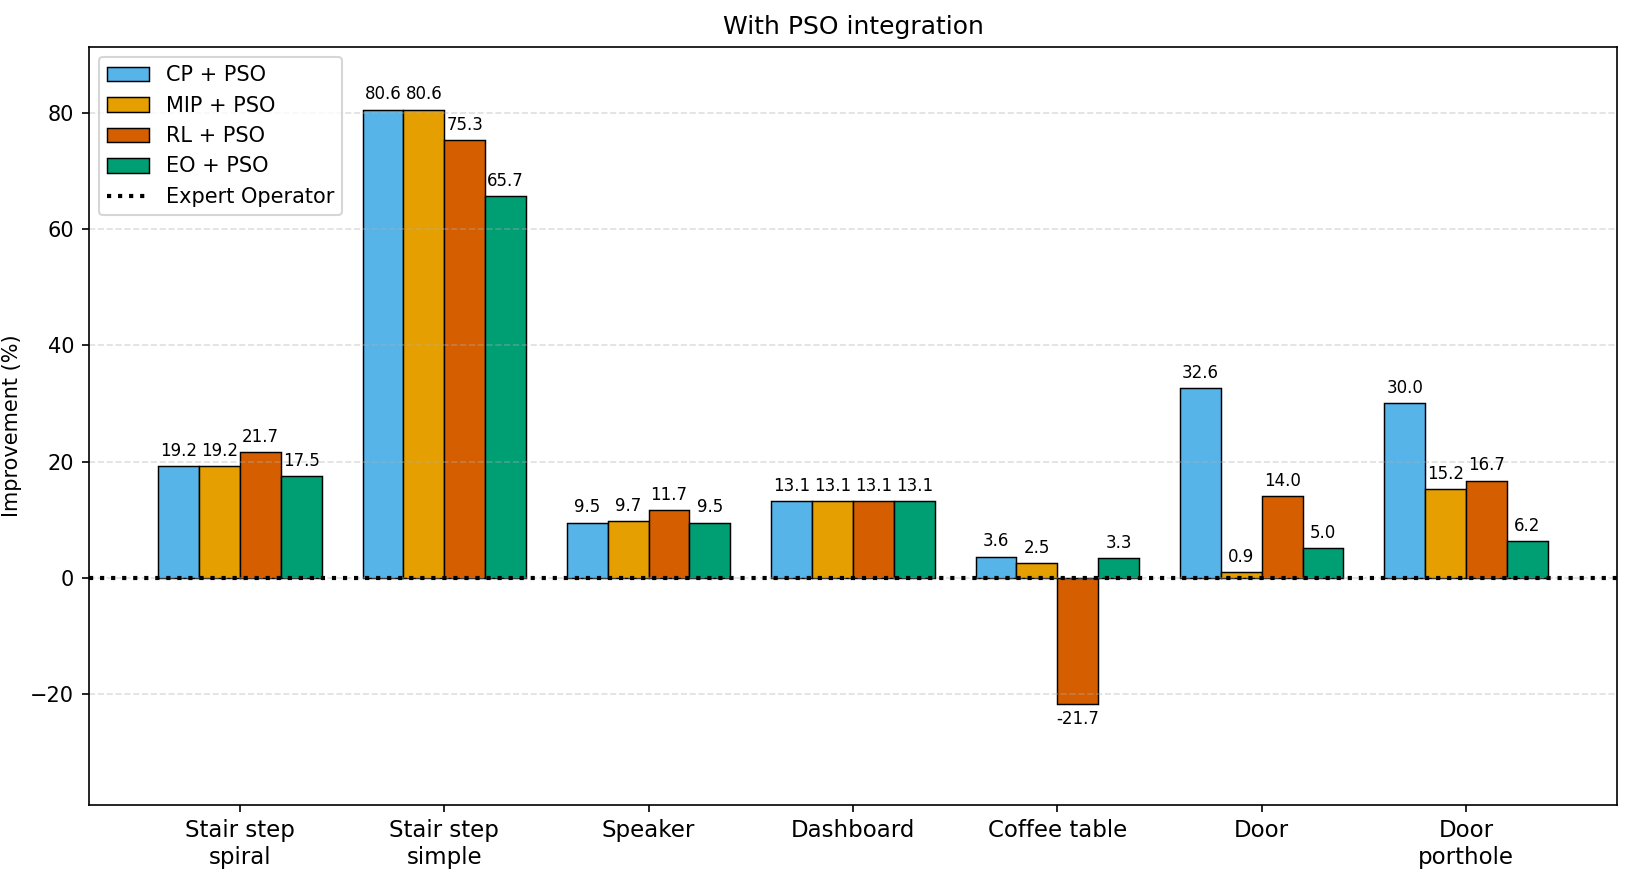
\includegraphics[width=0.7\textwidth]{img/comparison_plot_2.png}
		\caption{Percentage improvement over expert operator after PSO refinement}
		\label{fig:comparision_plot2}
	\end{subfigure}
	\caption{Percentage improvement relative to the solution provided by the expert operator. The first plot illustrates the improvements achieved by the CP model, MIP model and Q-learning algorithm without PSO integration, whereas the second plot presents the improvements obtained with PSO integration, alongside the improvement of the expert operator's solution when combined with PSO.}
	\label{fig:improvement}
\end{figure}

%\begin{figure}[t]
%	\centering
%	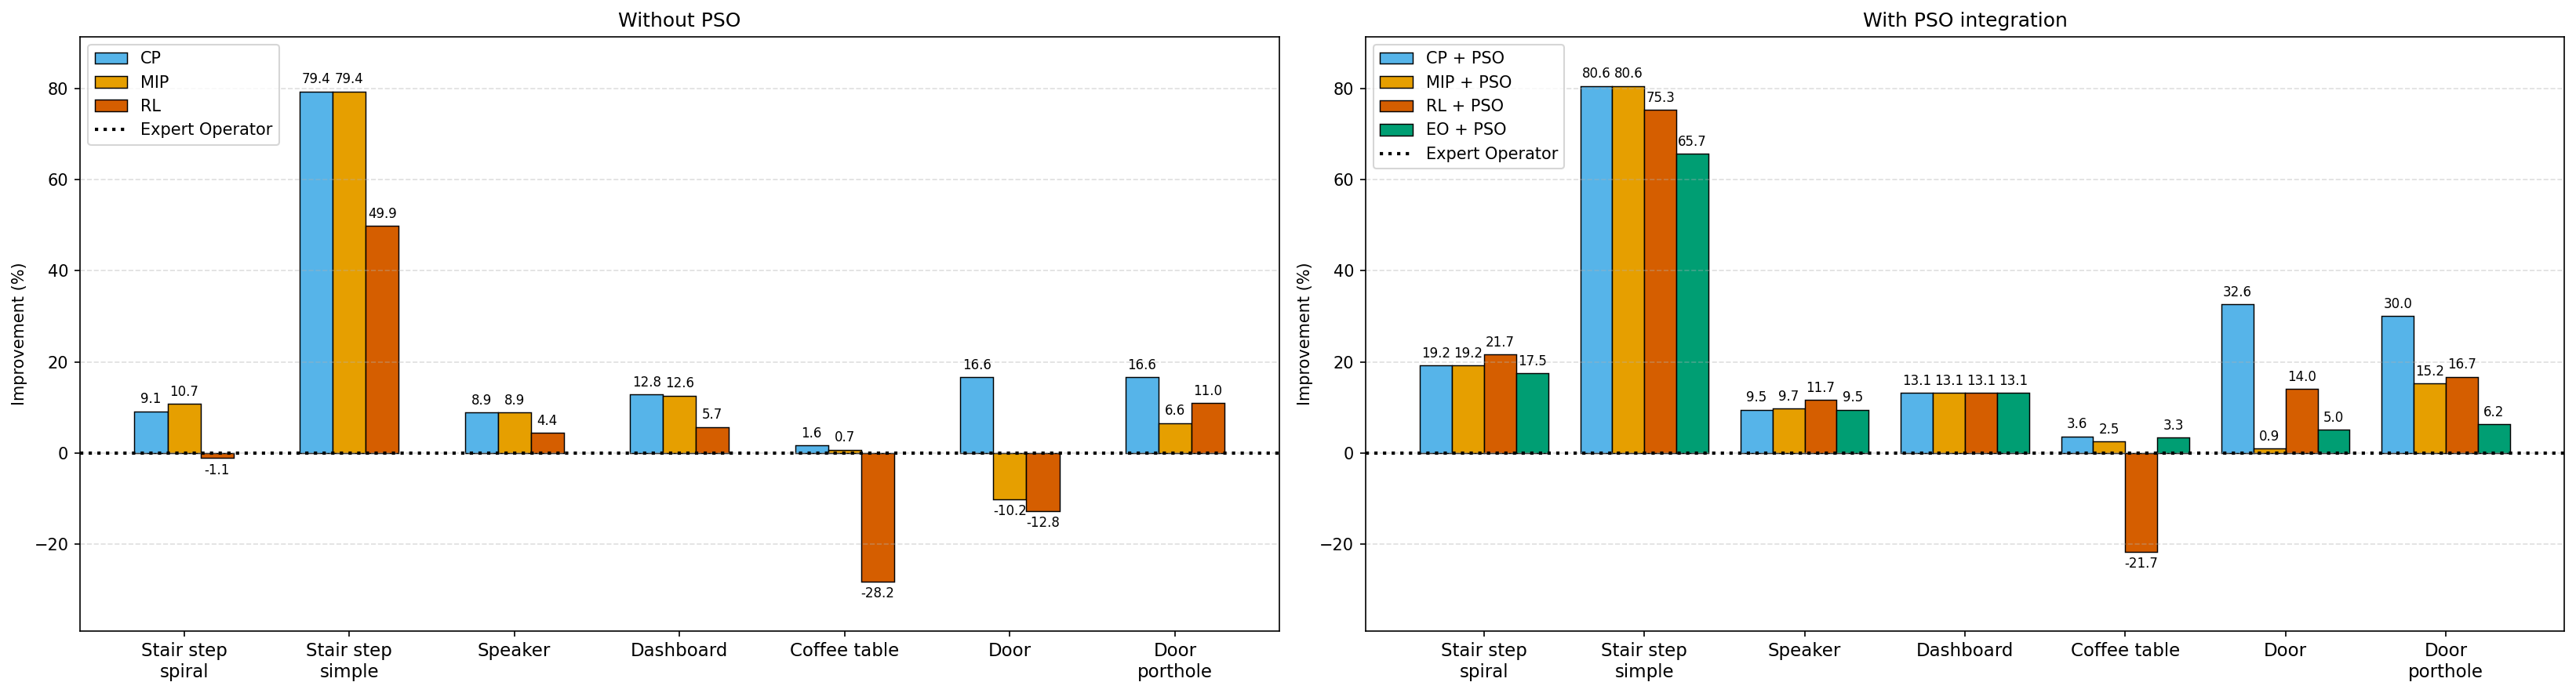
\includegraphics[width=\linewidth]{img/comparison_plot.png}
%	\caption{
%		Percentage improvement relative to the solution provided by the expert operator. The left plot illustrates the improvements achieved by the CP model, MIP model and Q-learning algorithm without PSO integration, whereas the right plot presents the improvements obtained with PSO integration, alongside the improvement of the expert operator's solution when combined with PSO.
%	}
%	\label{fig:improvement}
%\end{figure}

For each workpiece, the best CP and MIP solutions in terms of $\finer$, together with the Q-learning solution, were used as initial ones for the PSO algorithm. 

To enable direct integration into the target industrial system, the PSO algorithm was implemented in Java~18.0.2. Its hyper-parameters were tuned using the Optuna framework~\cite{akiba2019optuna}, yielding the following configuration: $\swarmsize = 1374$, $\maxiter = 2912$, $w = 0.669$, $c_1 = 2.385$, and $c_2 = 0.558$.

Figure~\ref{fig:improvement} shows the percentage improvement in $\finer$ with respect to the layout proposed by an expert operator. The first plot (Fig~\ref{fig:comparison_plot1}) reports the improvements achieved by the CP model, the MIP model, and the Q-learning algorithm before PSO refinement, whereas the second plot (Fig~\ref{fig:comparison_plot2}) shows the corresponding results after PSO refinement, including those obtained by initializing PSO from the expert layout.

The largest workpieces, namely the coffee table, the door, and the door with porthole, represent the most challenging instances. Among the considered approaches, the CP model consistently achieves the best improvements over the expert layout and is the only one that improves upon the expert solution for the door workpiece.

The Q-learning algorithm outperforms the expert layout in four of the seven considered workpieces. The integration with PSO further improves the solutions generated by the Q-learning algorithm for the stair step of the spiral staircase and the door, allowing them to surpass the expert layout. Conversely, starting from the Q-learning solution for the coffee table, only marginal improvements are obtained, highlighting the importance of starting the PSO search from a high-quality initial solution.

\begin{table}[!t]
	\centering
	\renewcommand{\arraystretch}{1.3}
	\setlength{\tabcolsep}{3pt}
	\caption{Summary of the best solutions, corresponding solution providers, and moment of inertia values for the different workpieces. 
		The workpiece perimeter is shown with solid lines. Dashed lines indicate extrusion areas, fixture regions are marked with diagonal hatching, and supporting bars are shown as shaded rectangles.}
	\label{tab:visual_results}
	\begin{tabular}{c c c c c}
		\hline
		\textbf{Workpiece} & \textbf{Expert Operator} & \textbf{Best CP/MIP} & \textbf{Q-learning} & \textbf{Best with PSO} \\
		\hline
		\makecell{Spiral stair step} & \makecell{$1.96057\times 10^{9}$ \\ 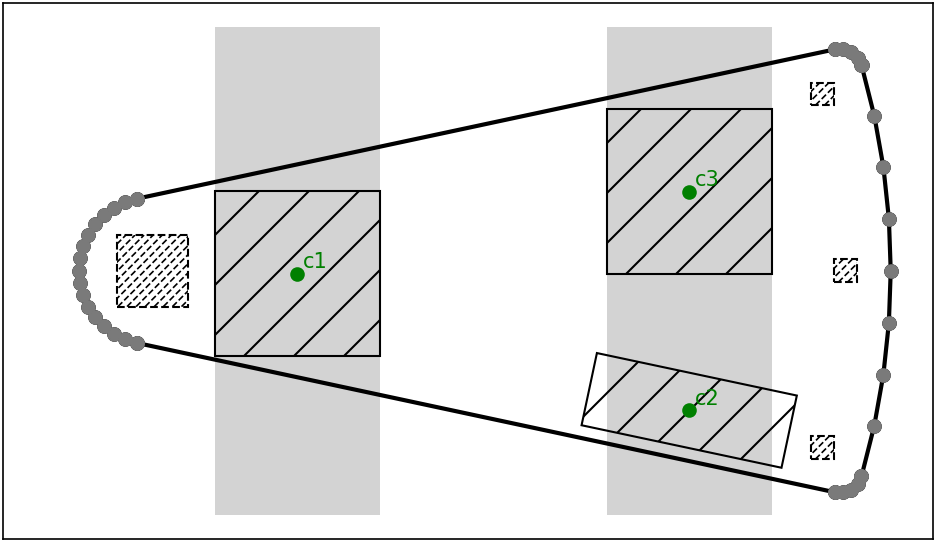
\includegraphics[width=0.18\linewidth]{img/spiral_stair_step_expert_operator.png}} & \makecell{MIP: $2.17089\times 10^{9}$ \\ 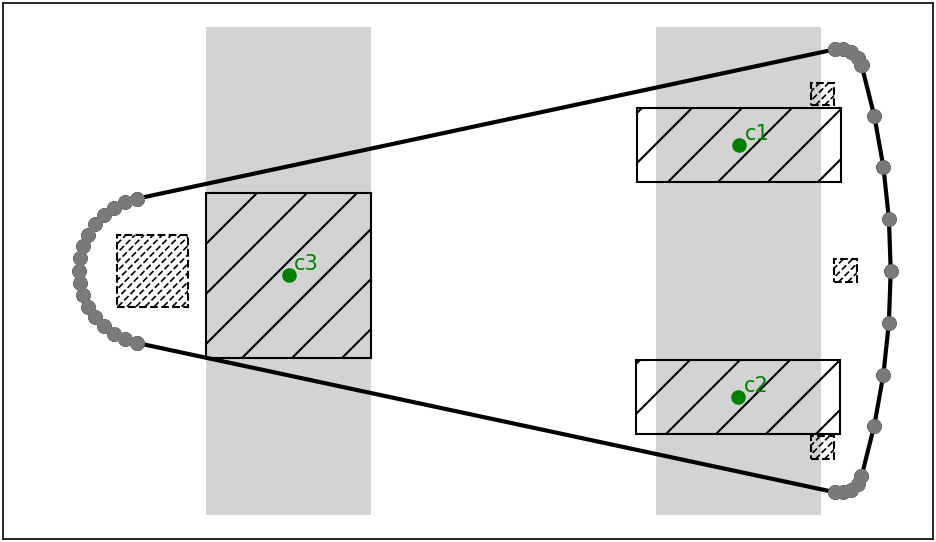
\includegraphics[width=0.18\linewidth]{img/spiral_stair_step_mip_model_gurobi.png}} & \makecell{$1.93822\times 10^{9}$ \\ 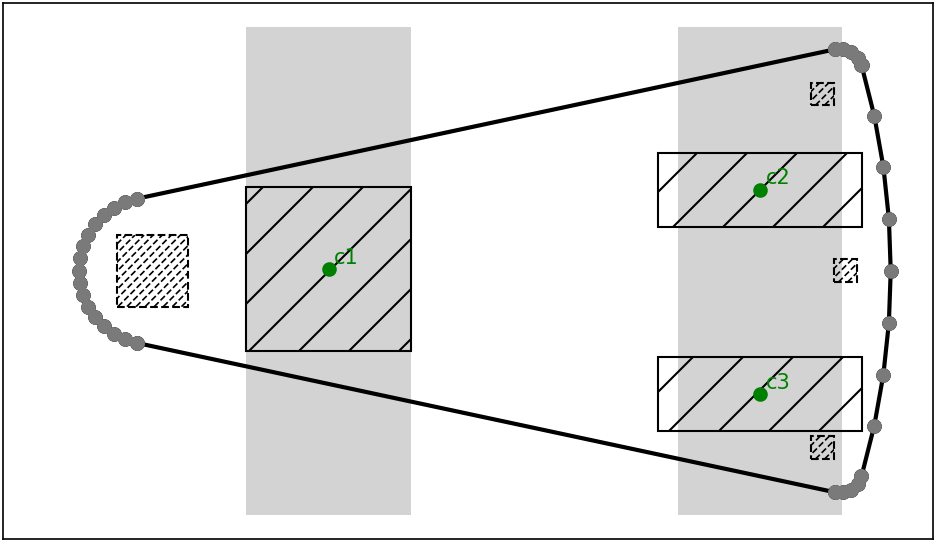
\includegraphics[width=0.18\linewidth]{img/spiral_stair_step_rl.png}} & \makecell{RL: $2.38520\times 10^{9}$ \\ 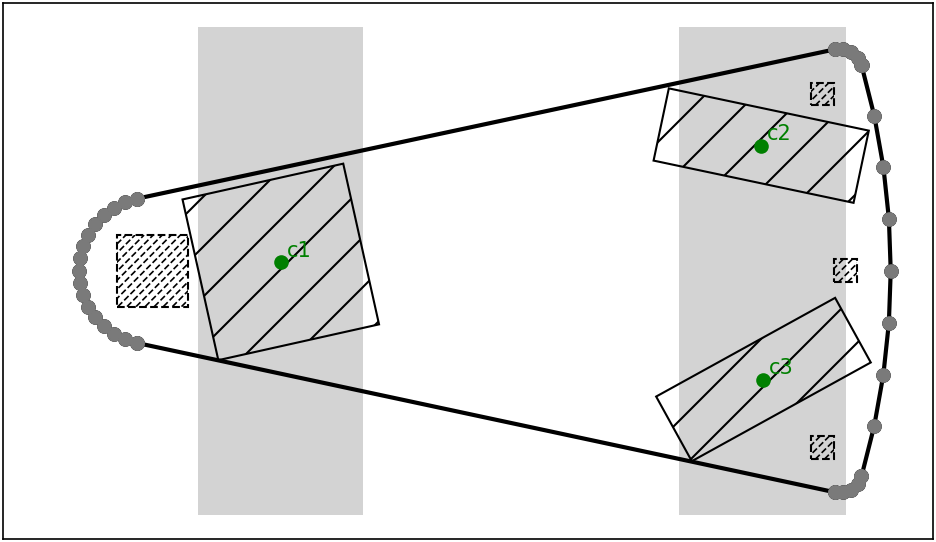
\includegraphics[width=0.18\linewidth]{img/spiral_stair_step_pso_rl_pso.png}} \\
		\hline
		\makecell{Simple stair step} & \makecell{$3.77213\times 10^{9}$ \\ 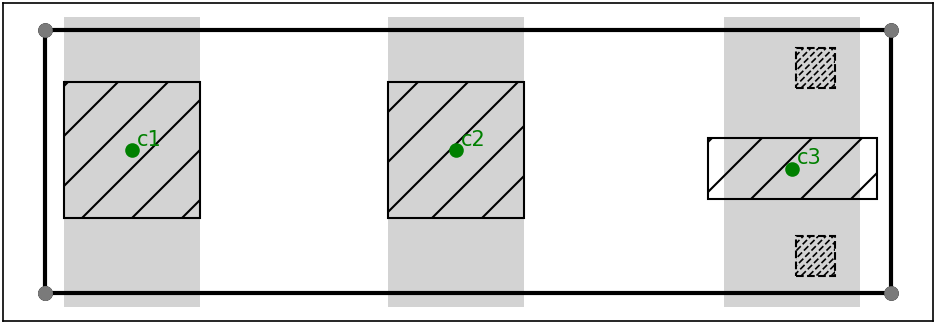
\includegraphics[width=0.18\linewidth]{img/simple_stair_step_expert_operator.png}} & \makecell{MIP: $6.76638\times 10^{9}$ \\ 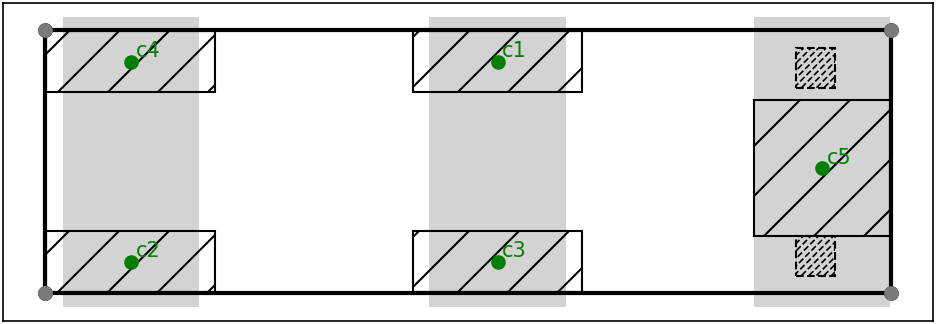
\includegraphics[width=0.18\linewidth]{img/simple_stair_step_mip_model_gurobi.png}} & \makecell{$5.65433\times 10^{9}$ \\ 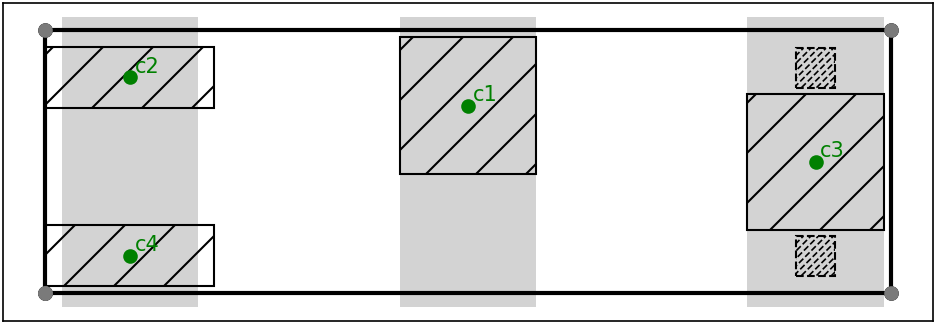
\includegraphics[width=0.18\linewidth]{img/simple_stair_step_rl.png}} & \makecell{CP: $6.81108\times 10^{9}$ \\ 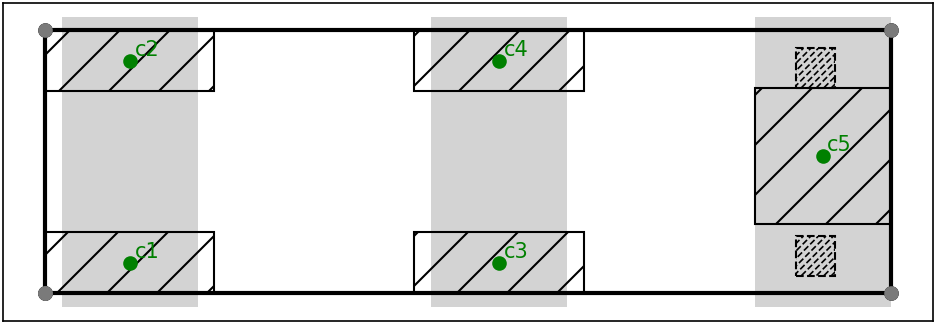
\includegraphics[width=0.18\linewidth]{img/simple_stair_step_pso_cp_pso.png}} \\
		\hline
		\makecell{Dashboard} & \makecell{$6.29544\times 10^{9}$ \\ 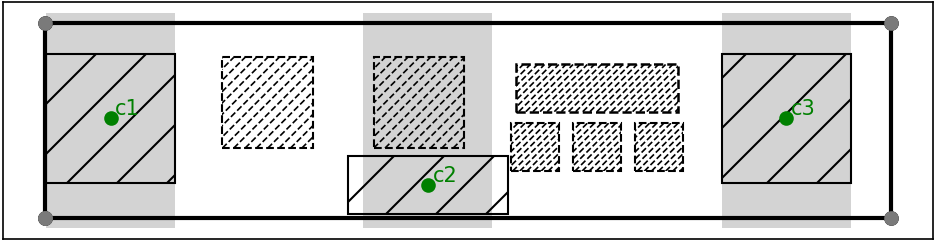
\includegraphics[width=0.18\linewidth]{img/dashboard_expert_operator.png}} & \makecell{CP: $7.10094\times 10^{9}$ \\ 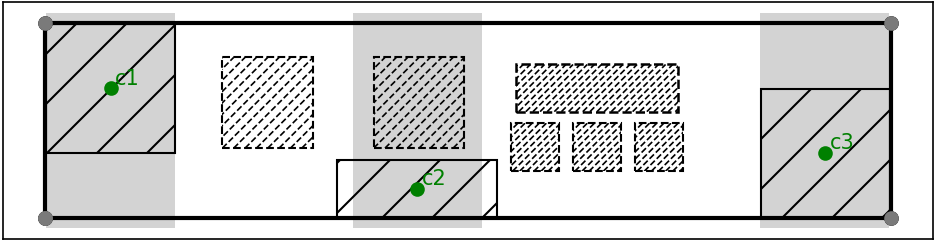
\includegraphics[width=0.18\linewidth]{img/dashboard_cp_model_gecode.png}} & \makecell{$6.65446\times 10^{9}$ \\ 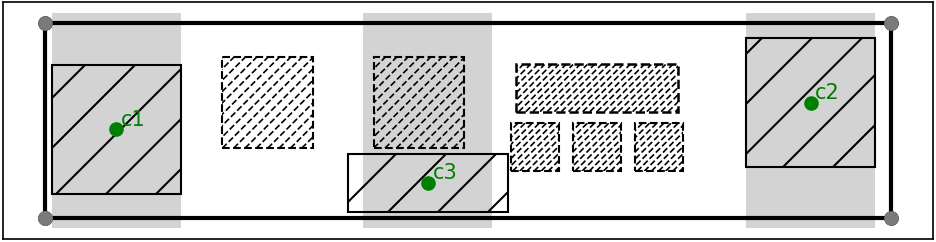
\includegraphics[width=0.18\linewidth]{img/dashboard_rl.png}} & \makecell{CP: $7.12226\times 10^{9}$ \\ 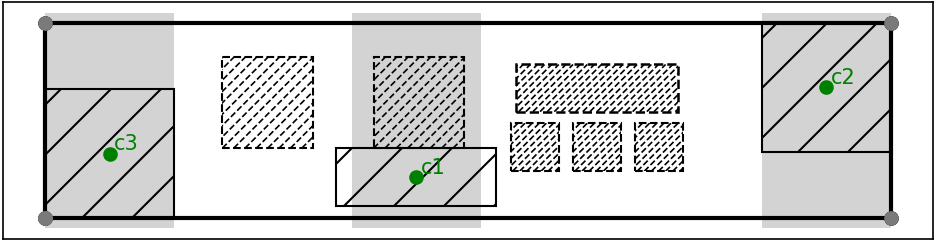
\includegraphics[width=0.18\linewidth]{img/dashboard_pso_cp_pso.png}} \\
		\hline
		\makecell{Speaker} & \makecell{$2.69490\times 10^{9}$ \\ 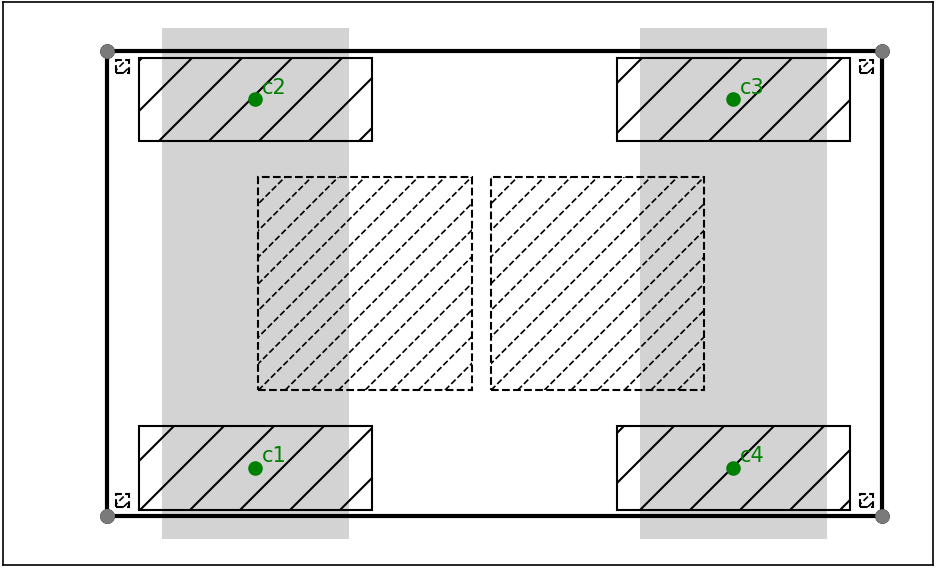
\includegraphics[width=0.18\linewidth]{img/speaker_expert_operator.png}} & \makecell{CP, MIP: $2.93433\times 10^{9}$ \\ 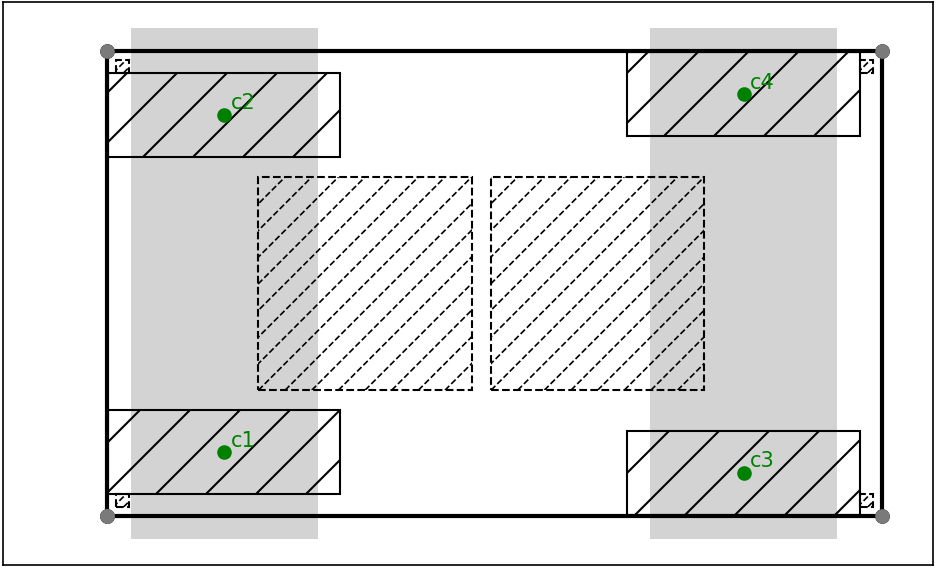
\includegraphics[width=0.18\linewidth]{img/speaker_cp_model_gecode.png}} & \makecell{$2.81248\times 10^{9}$ \\ 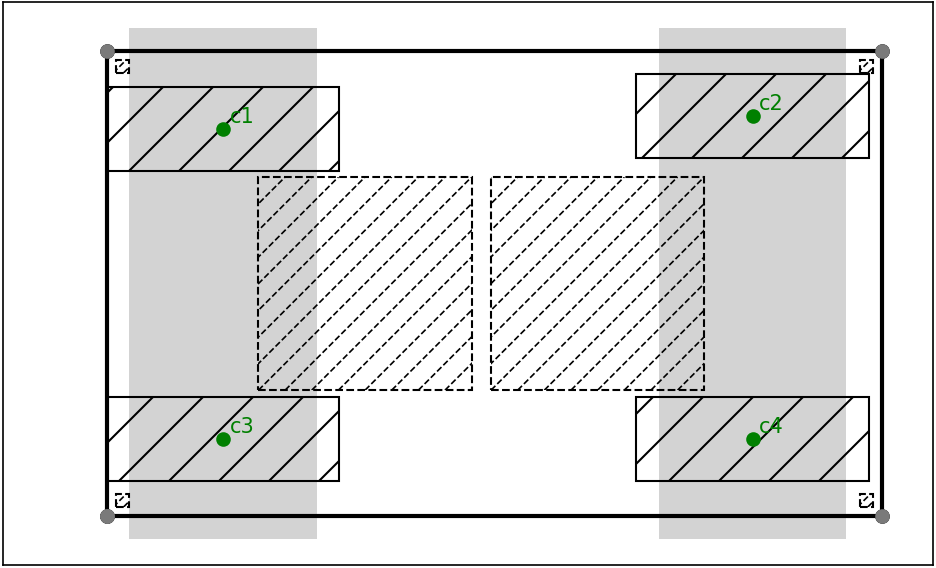
\includegraphics[width=0.18\linewidth]{img/speaker_rl.png}} & \makecell{RL: $3.00979\times 10^{9}$ \\ 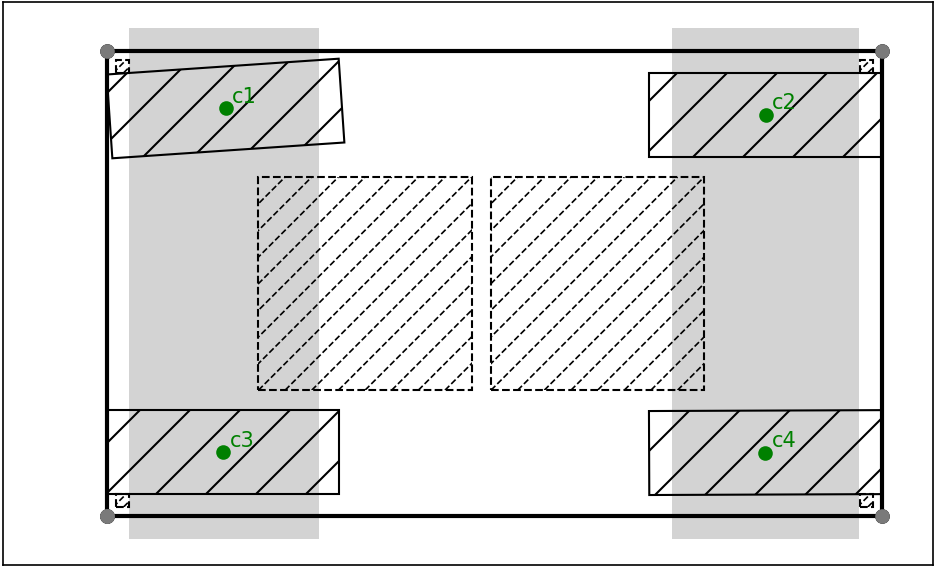
\includegraphics[width=0.18\linewidth]{img/speaker_pso_rl_pso.png}} \\
		\hline
		\makecell{Coffee table} & \makecell{$2.17954\times 10^{10}$ \\ 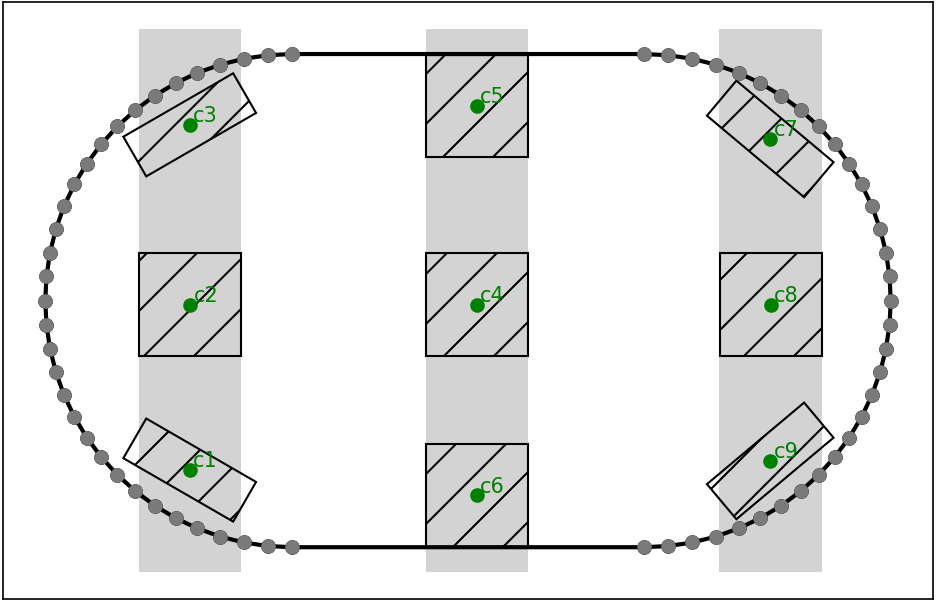
\includegraphics[width=0.18\linewidth]{img/coffee_table_expert_operator.png}} & \makecell{CP: $2.21449\times 10^{10}$ \\ 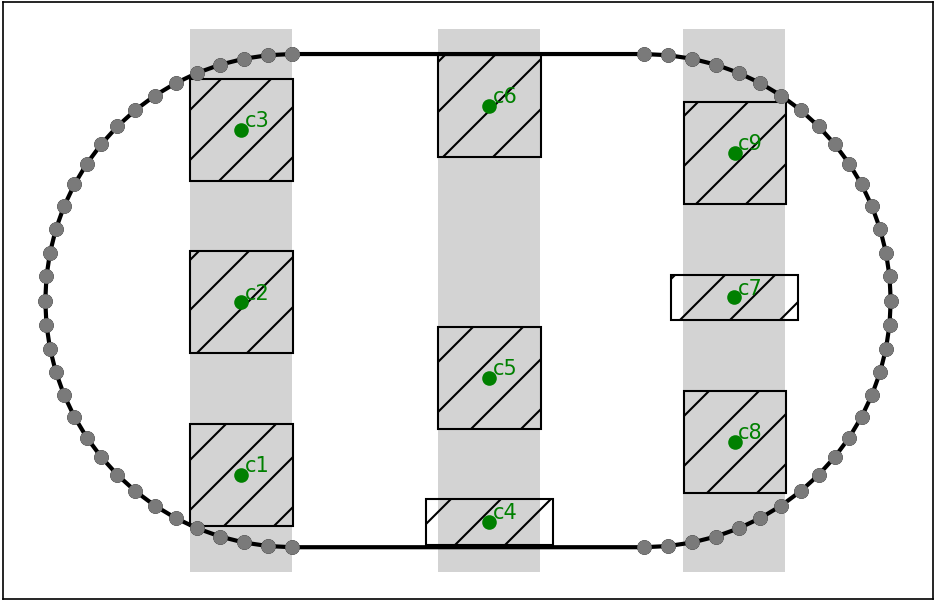
\includegraphics[width=0.18\linewidth]{img/coffee_table_cp_model_chuffed.png}} & \makecell{$1.56444\times 10^{10}$ \\ 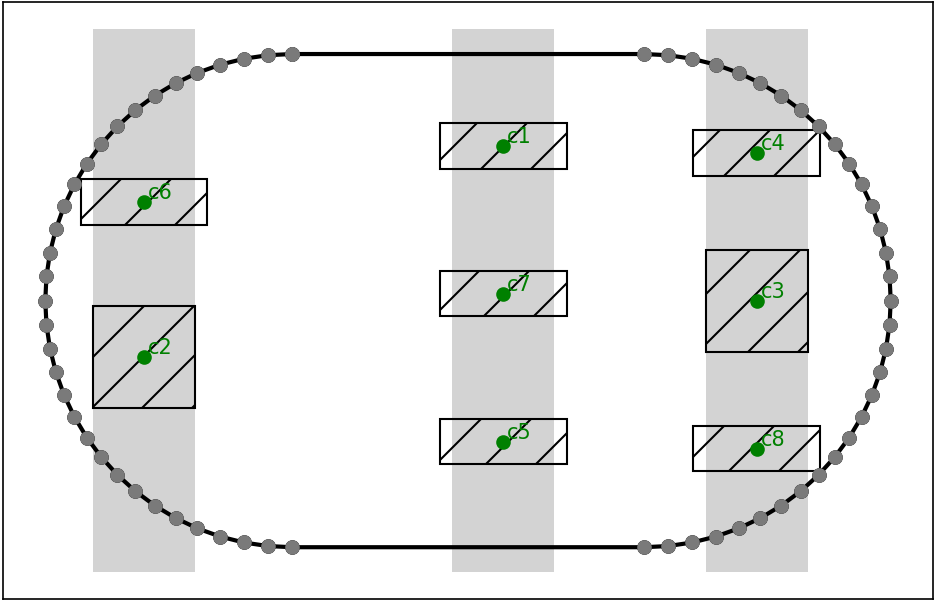
\includegraphics[width=0.18\linewidth]{img/coffee_table_rl.png}} & \makecell{CP: $2.25868\times 10^{10}$ \\ 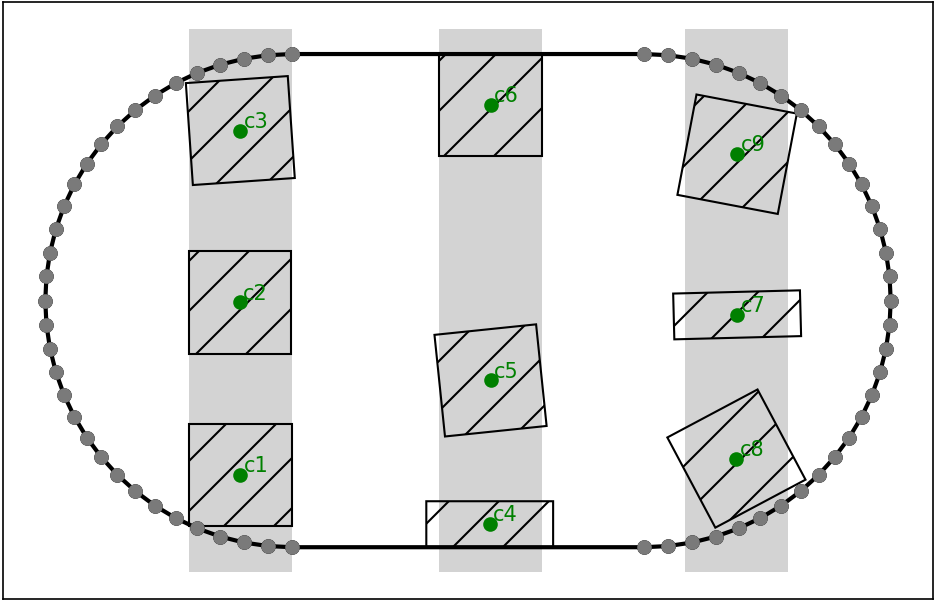
\includegraphics[width=0.18\linewidth]{img/coffee_table_pso_cp_pso.png}} \\
		\hline
		\makecell{Door} & \makecell{$1.31109\times 10^{11}$ \\ 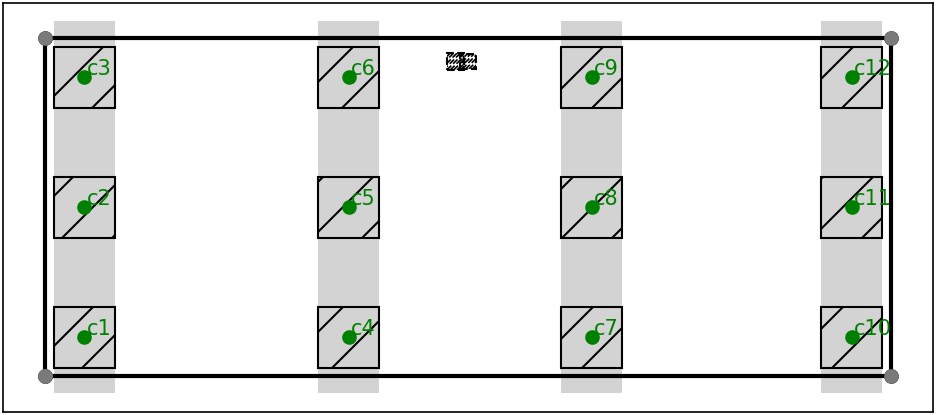
\includegraphics[width=0.18\linewidth]{img/door_expert_operator.png}} & \makecell{CP: $1.52925\times 10^{11}$ \\ 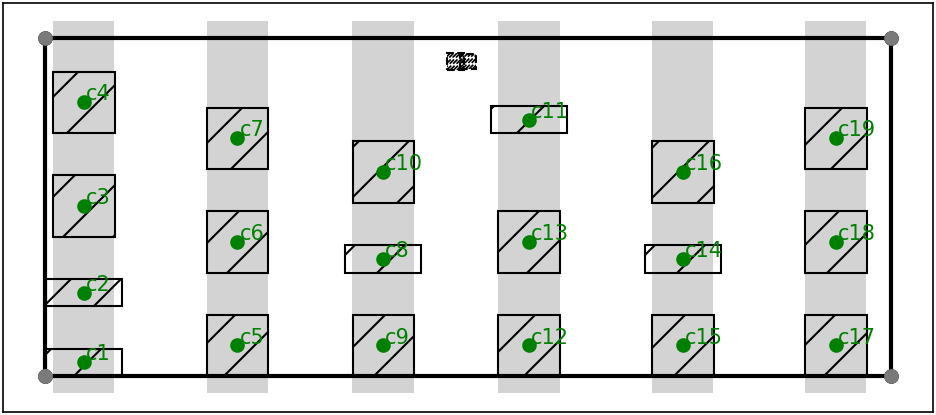
\includegraphics[width=0.18\linewidth]{img/door_LNS_cp_model_gecode.png}} & \makecell{$1.14387\times 10^{11}$ \\ 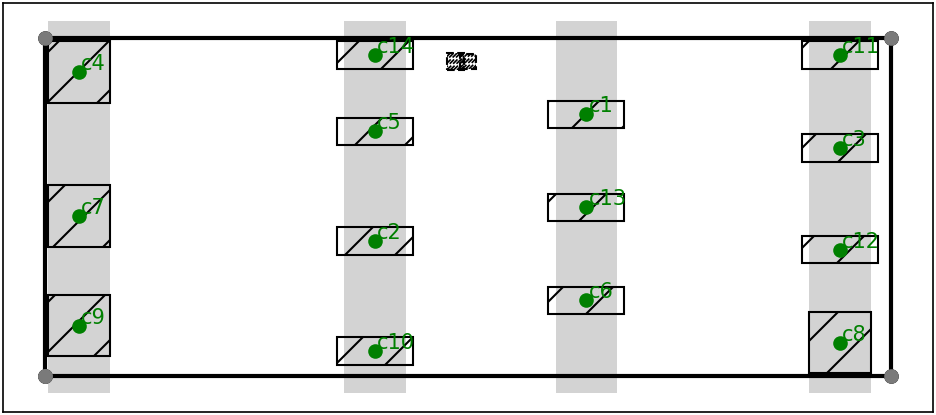
\includegraphics[width=0.18\linewidth]{img/door_rl.png}} & \makecell{CP: $1.73826\times 10^{11}$ \\ 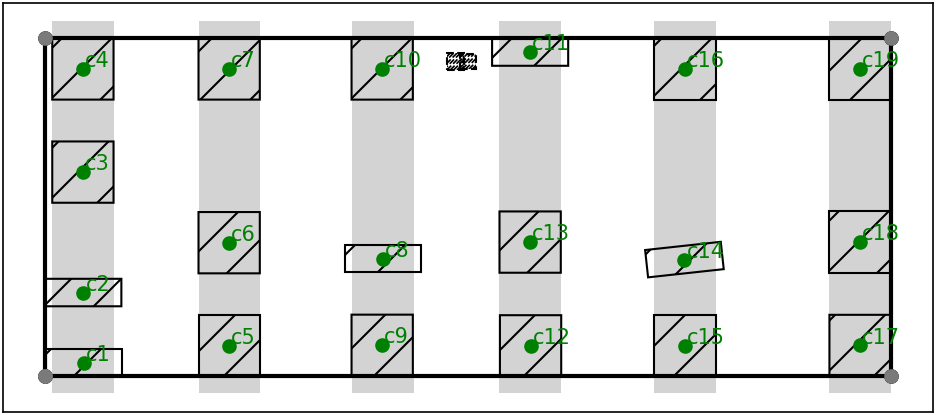
\includegraphics[width=0.18\linewidth]{img/door_pso_cp_pso.png}} \\
		\hline
		\makecell{Door porthole} & \makecell{$1.31109\times 10^{11}$ \\ 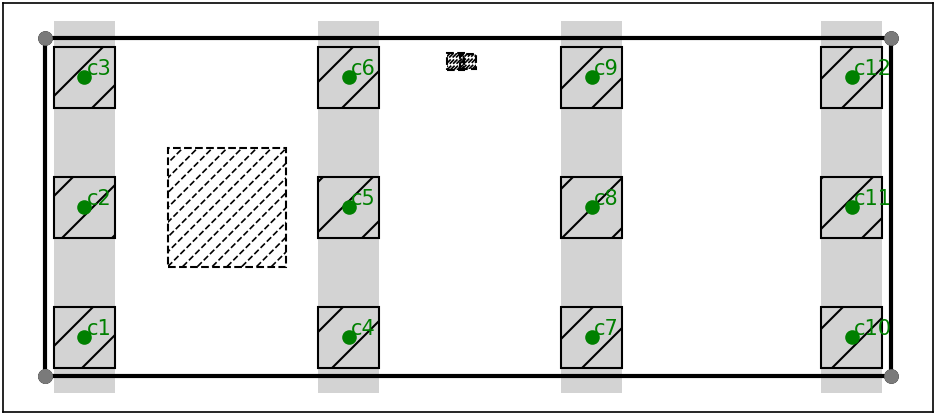
\includegraphics[width=0.18\linewidth]{img/door_porthole_expert_operator.png}} & \makecell{CP: $1.52861\times 10^{11}$ \\ 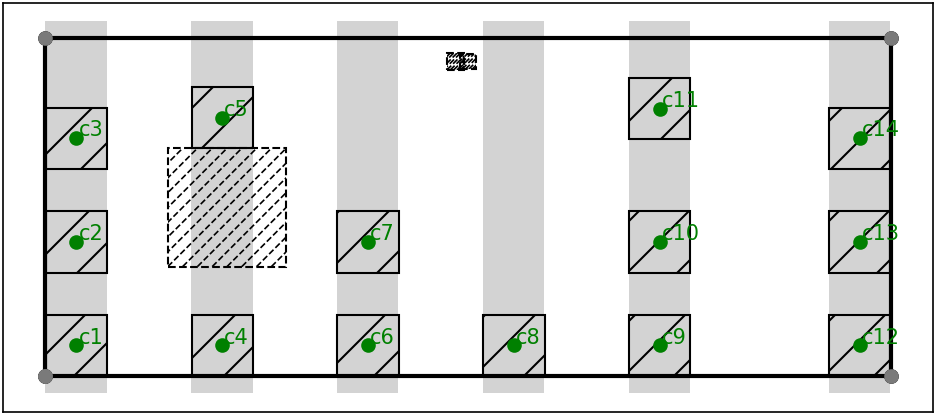
\includegraphics[width=0.18\linewidth]{img/door_porthole_LNS_cp_model_gecode.png}} & \makecell{$1.45467\times 10^{11}$ \\ 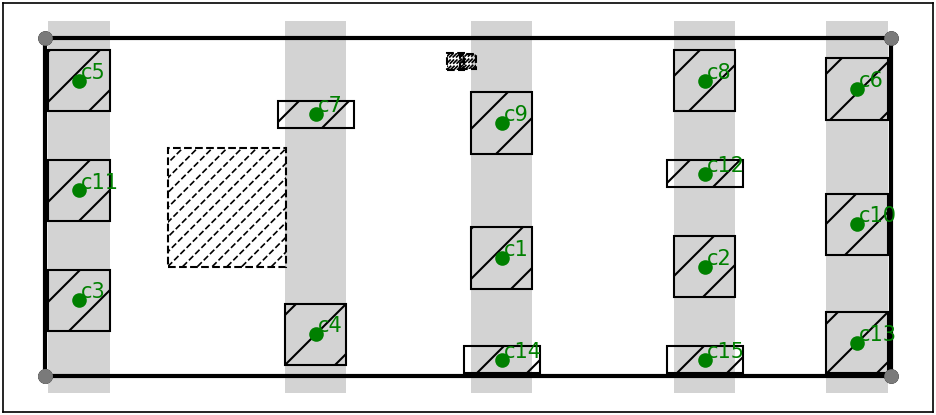
\includegraphics[width=0.18\linewidth]{img/door_porthole_rl.png}} & \makecell{CP: $1.70507\times 10^{11}$ \\ 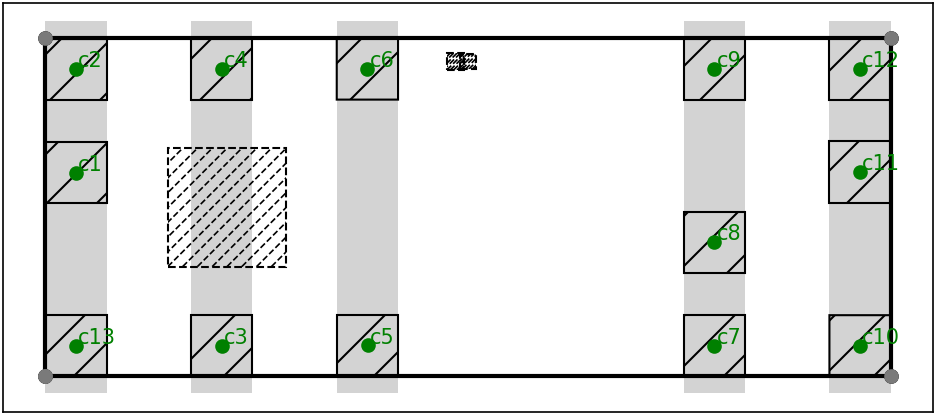
\includegraphics[width=0.18\linewidth]{img/door_porthole_pso_cp_pso.png}} \\
		\hline
	\end{tabular}
\end{table}


Table~\ref{tab:visual_results} reports visual comparisons of the best solutions obtained with the CP model, the MIP model, and the Q-learning algorithm for the different workpieces, together with the corresponding solutions refined by PSO. Note that, in the figures, the support bars can be positioned beneath the extrusion areas, since the fixture height prevents collisions between the cutting tools and the bars.

The layouts proposed by the Q-learning algorithm are qualitatively similar to those obtained with the CP and MIP models. An exception is the coffee table, where Q-learning tends to favour the placement of a larger number of rectangular fixtures instead of square ones, resulting in a lower value for the moment of inertia.

Rotation plays an important role in the stair step of the spiral staircase and coffee table workpieces, where fixture orientation improves adherence to the workpiece boundary. For the Speaker workpiece, the PSO refinement of the Q-learning solution introduces only a slight rotation of the upper-left fixture, yielding the marginal improvement reported in Figure~\ref{fig:improvement}.

The Stair step of the simple staircase exhibits the largest improvement over the expert layout. This is mainly due to the use of a larger number of fixtures, five for the CP and MIP models and four for the Q-learning algorithm, compared with the three fixtures used by the expert operator.

For both the door and the door with a porthole workpieces, the expert operator adopts a symmetric fixture layout, whereas the PSO refinement tends to move the fixtures farther from the workpiece centre. Since the principal moments of inertia are maximised when the fixtures are placed away from the symmetry axes, this configuration yields higher values of $\finer$. Moreover, in the door workpiece, the expert layout relies exclusively on square fixtures, whereas the optimization strategies increase the number of fixtures using even rectangular ones, thereby increasing the supported area of the workpiece.

Overall, the best trade-off between computational time and solution quality is achieved by integrating the CP model with PSO. Moreover, the CP formulation is expected to scale better to problems involving additional fixture types and multiple extrusion areas owing to the stronger propagation of the \texttt{diffn} global constraint and the fact that type and overlap decisions are modeled through discrete variables that cannot be relaxed, unlike the $x$ and $y$ variables in the MIP formulation.

